
\begin{figure}[!htb]
\begin{center}
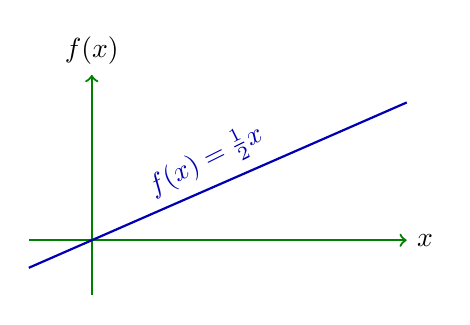
\begin{tikzpicture}
[
	xscale	= 0.8,	% to scale horizontally everything but the text
	yscale	= 0.7,	% to scale vertically everything but the text
]


\draw [->, color=black!50!green, thick] (-1,0) -- (5,0) node [right, color=black] {$x$};
\draw [->, color=black!50!green, thick] (0,-1) -- (0,3) node [above, color=black] {$f(x)$};
\draw [-, color=blue!70!black, thick] (-1,-0.5) -- (5,2.5) node [midway, above, sloped] {$f(x) = \frac{1}{2} x$};


\end{tikzpicture}
\end{center}
\end{figure}
 
